\documentclass[11pt,a4paper]{article}
\usepackage[utf8]{inputenc}
\usepackage[spanish]{babel}	%Idioma
\usepackage{amsmath}
\usepackage{amsfonts}
\usepackage{amssymb}
\usepackage{graphicx} 	%Añadir imágenes
\usepackage{geometry}	%Ajustar márgenes
\usepackage[export]{adjustbox}[2011/08/13]
\usepackage{float}
\restylefloat{table}
\usepackage[hidelinks]{hyperref}
\usepackage{titling}
\usepackage{multirow}
\usepackage{caption}
\usepackage{multicol}
\usepackage[shortlabels]{enumitem}
\usepackage{array}
\selectlanguage{spanish}

%Opciones de encabezado y pie de página:
\usepackage{fancyhdr}
\pagestyle{fancy}
\lhead{Nazaret Román Guerrero}
\rhead{Sistemas Gráficos}
\lfoot{Grado en Ingeniería Informática}
\cfoot{}
\rfoot{\thepage}
\renewcommand{\headrulewidth}{0.4pt}
\renewcommand{\footrulewidth}{0.4pt}

%Opciones de fuente:
\usepackage[utf8]{inputenc}
\usepackage[default]{sourcesanspro}
\usepackage{sourcecodepro}
\usepackage[T1]{fontenc}

\setlength{\parindent}{15pt}
\setlength{\headheight}{15pt}
\setlength{\voffset}{10mm}

% Custom colors
\usepackage{color}
\definecolor{deepblue}{rgb}{0,0,0.5}
\definecolor{deepred}{rgb}{0.6,0,0}
\definecolor{deepgreen}{rgb}{0,0.5,0}
\definecolor{morado}{rgb}{0.4,0,0.8}

\usepackage{listings}

\begin{document}
\begin{titlepage}

\begin{minipage}{\textwidth}

\centering
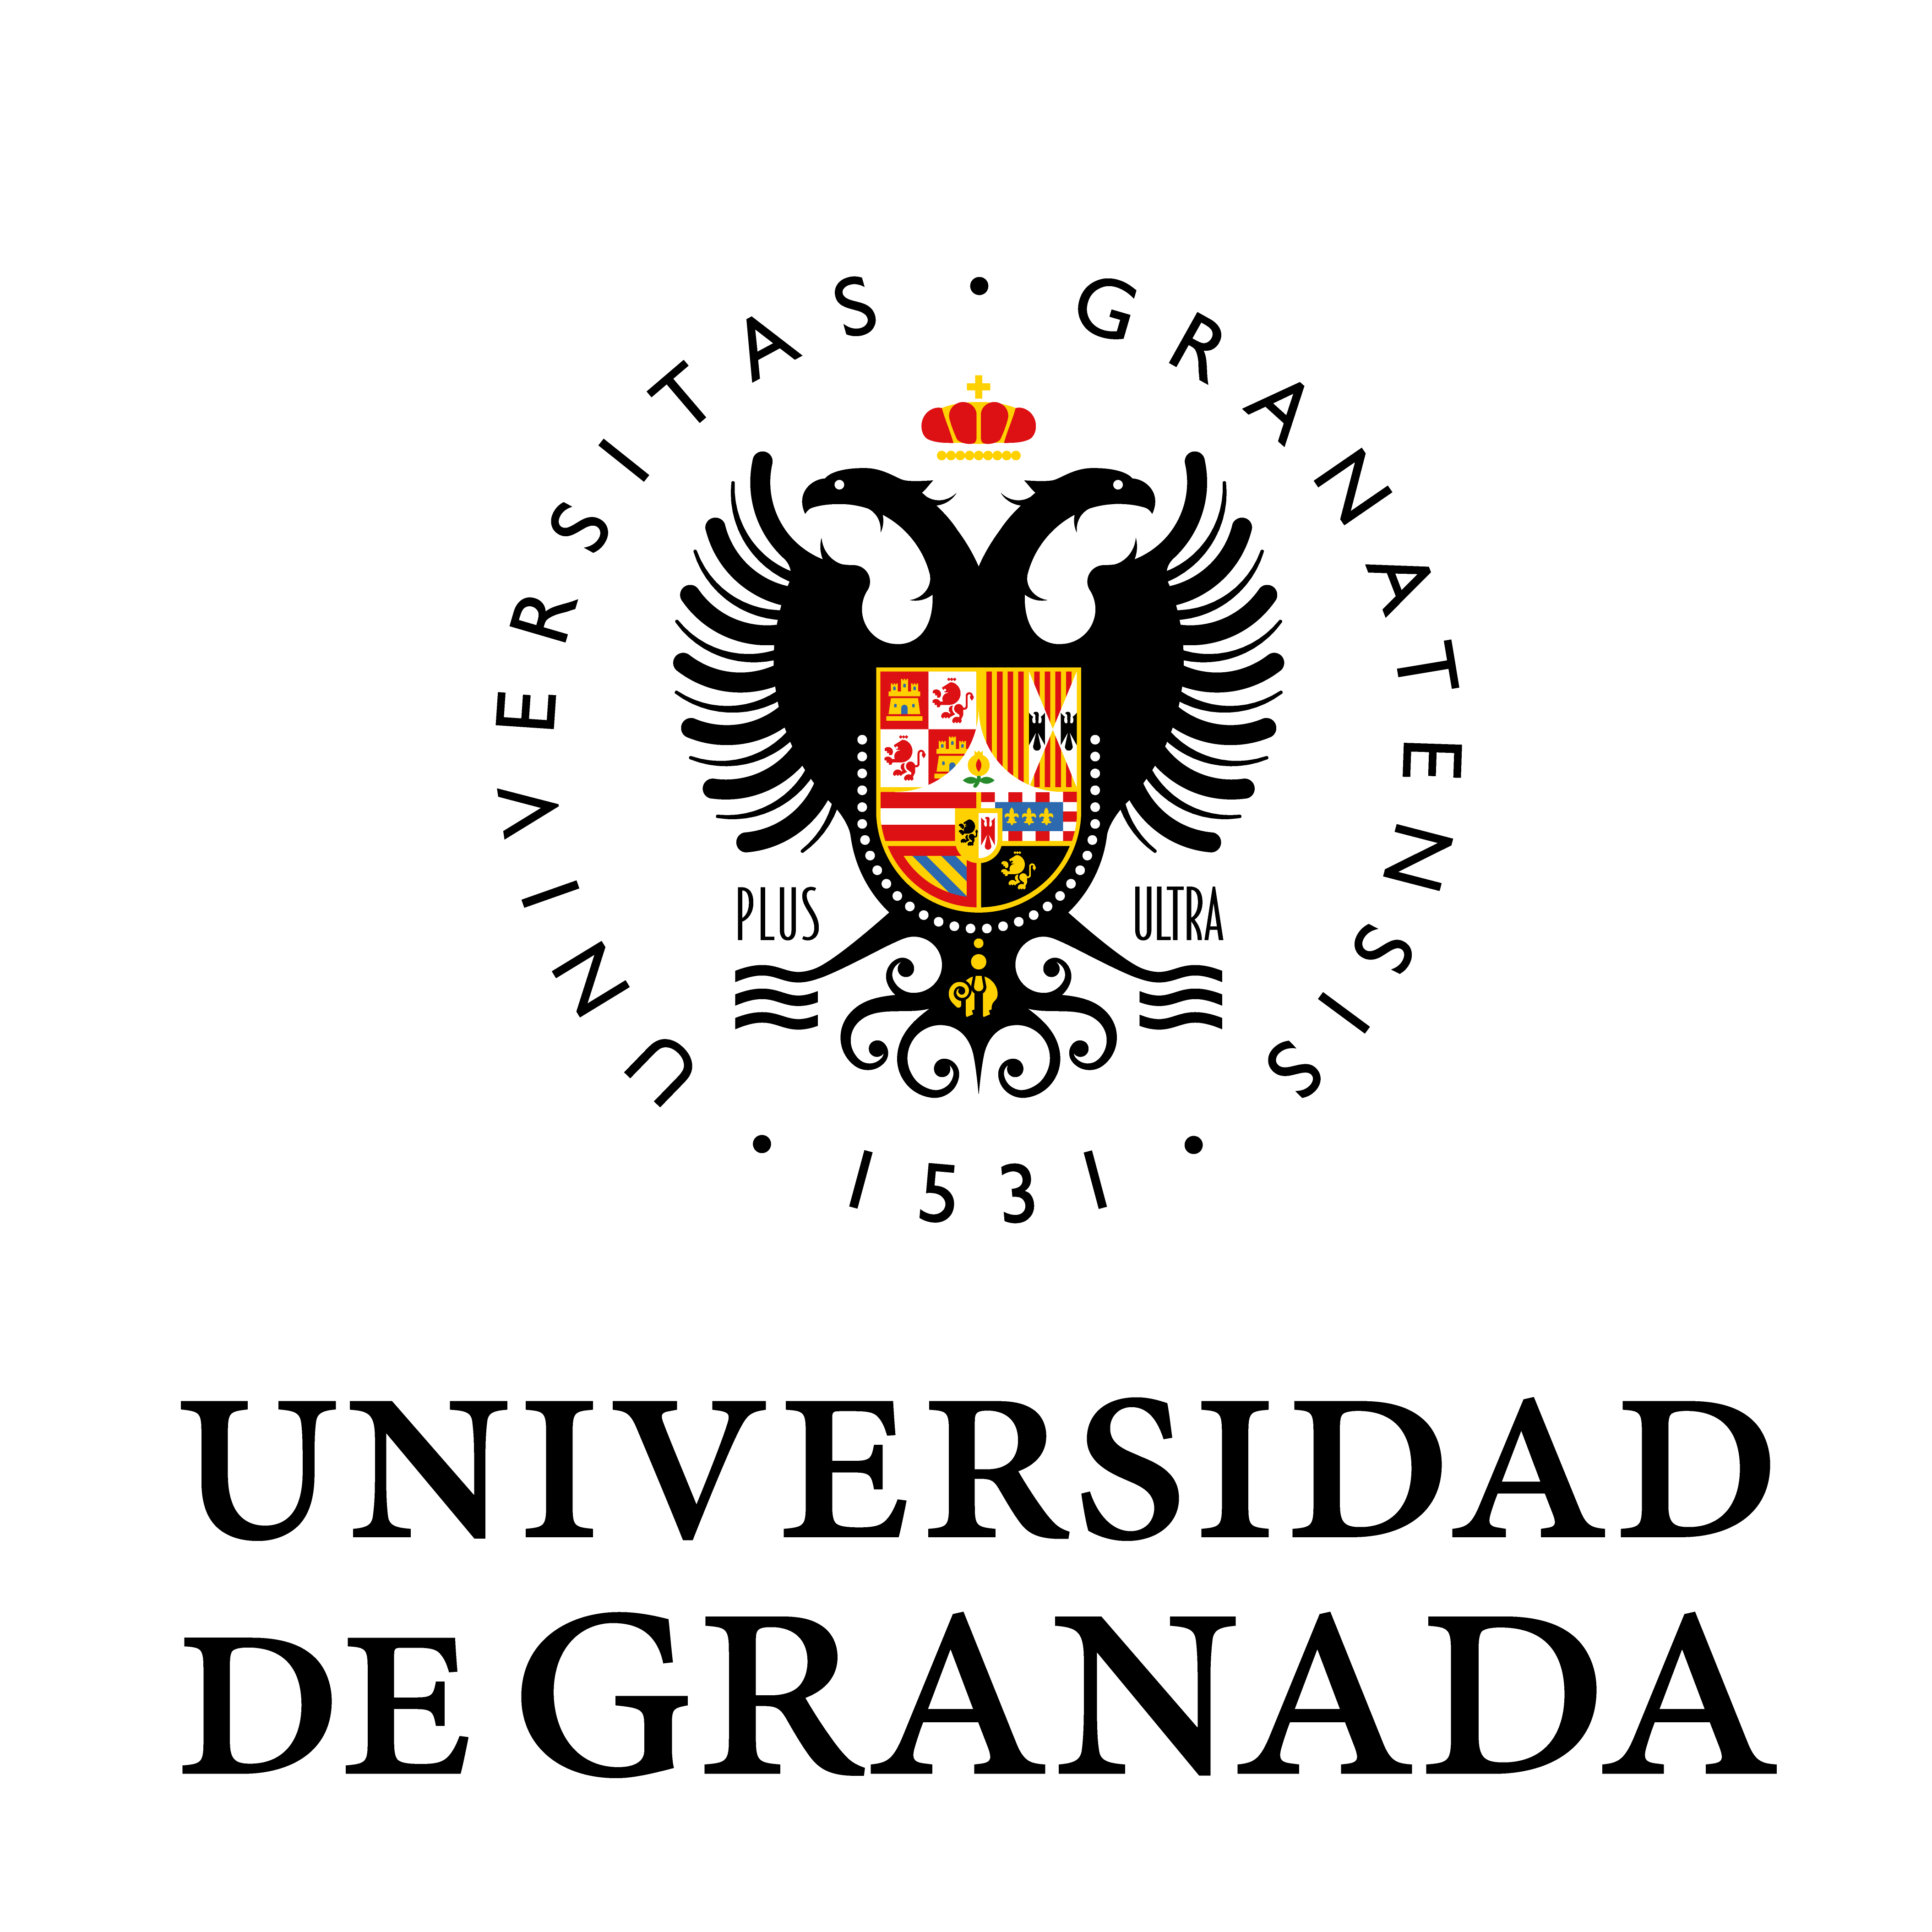
\includegraphics[width=0.5\textwidth]{img/logo.png}\\

\textsc{\Large Sistemas Gráficos\\[0.2cm]}
\textsc{GRADO EN INGENIERÍA INFORMÁTICA}\\[1cm]

{\Huge\bfseries Manual de usuario\\}
\noindent\rule[-1ex]{\textwidth}{3pt}\\[3.5ex]
{\large\bfseries Bleach RPG}
\end{minipage}

\vspace{1.5cm}
\begin{minipage}{\textwidth}
\centering

\textbf{Autora}\\ {Nazaret Román Guerrero}\\[2.5ex]

\includegraphics[width=0.3\textwidth]{img/etsiit.jpeg}\\[0.1cm]
\vspace{1cm}
\textsc{Escuela Técnica Superior de Ingenierías Informática y de Telecomunicación}\\
\vspace{1cm}
\textsc{Curso 2019-2020}
\end{minipage}
\end{titlepage}

\pagenumbering{gobble}
\pagenumbering{arabic}

\newpage

\section{Objetivo del juego}

Nos encontramos ante un juego de rol (Rol-Play Game, RPG) donde nos encontramos con Kurosaki Ichigo, nuestro personaje principal, vestido de negro.\\

Nuestra misión es enfrentarnos a nuestro enemigo, Grimmjow Jaegerjaquez, vestido de blanco y que está protegiendo una esfera que emite una tenue luz azul, rodeada por una caja semitransparente que la protege.\\

Esa esfera es el alma de Ichigo, que debe se recuperada puesto que se la han robado para convertirla en un arma. Si conseguimos matar a Grimmjow, recuperaremos el alma, pero si no lo derrotamos... Ichigo morirá.

\section{Cómo acceder a la pantalla del juego}

\section{Controles}

\subsection{Movimientos por la pantalla}

Para jugar debemos controlar los movimientos del personaje principal, llamado Kurosaki Ichigo. Nuestro personaje comienza en mitad del escenario, de espaldas a la cámara, tal y como vemos en la imagen:

\begin{figure}[H]
	\centering
	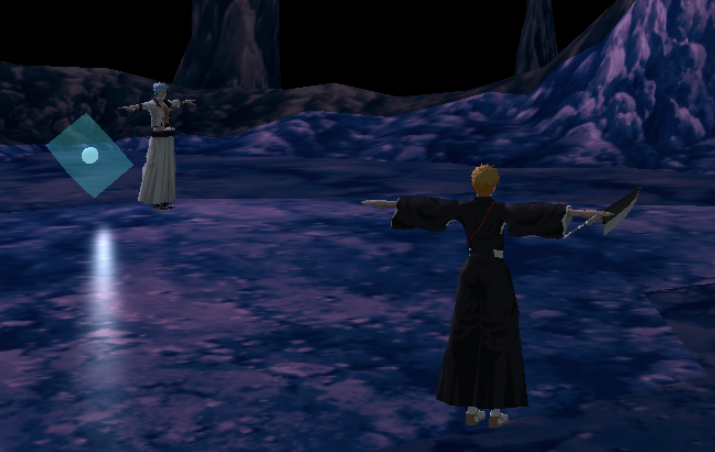
\includegraphics[scale=0.5]{img/inicio.png}
\end{figure}

Para mover a este personaje por el escenario es necesario moverlo con las teclas \color{morado}\texttt{asdw}\color{black}, de las cuales cada una significa lo siguiente:

	\begin{itemize}
		\item \color{morado}\texttt{a}\color{black}: el personaje se mueve hacia la izquierda.
		\item \color{morado}\texttt{s}\color{black}: el personaje se mueve hacia abajo (hacia fuera de la pantalla).
		\item \color{morado}\texttt{d}\color{black}: el personaje se mueve hacia la derecha.
		\item \color{morado}\texttt{w}\color{black}: el personaje se mueve hacia abajo (hacia dentro de la pantalla).
	\end{itemize}
	
\begin{figure}[H]
	\centering
	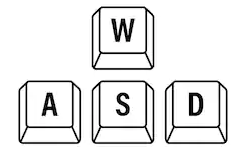
\includegraphics[scale=0.5]{img/teclas.png}
\end{figure}

\subsection{Atacar}

El personaje puede atacar mediante un click de ratón. No obstante, esto solo pasará cuando ambos personajes estén a distancia para colisionar; es decir, al pulsar el botón principal del ratón cuando el enemigo está en el rango de ataque le haremos daño. No obstante, también nos haremos daño nosotros, así que ¡cuidado!

\end{document}